\documentclass[aspectratio=169]{beamer}
\usetheme{Madrid}
\usecolortheme{default}

\usepackage{amsmath}
\usepackage{amssymb}
\usepackage{graphicx}
\usepackage{booktabs}
\usepackage{tikz}

\title{Magneto-Coulombic Actuation System \\ for Active Debris Removal}
\subtitle{A Propellantless Approach to LEO Sustainability}
\author{Research Hackathon Submission}
\institute{IIT Kanpur - Institute Research Symposium 2025}
\date{\today}

\begin{document}

\frame{\titlepage}

%% SECTION 1: PROBLEM STATEMENT
\begin{frame}{The Space Debris Crisis}
\textbf{Low Earth Orbit Congestion:}
\begin{itemize}
    \item 200-2,000 km altitude faces critical debris accumulation
    \item Defunct satellites, rocket bodies, collision fragments
    \item \textcolor{red}{\textbf{Kessler Syndrome}} threat: cascading collisions
\end{itemize}

\vspace{0.3cm}
\textbf{Mega-Constellation Impact:}
\begin{itemize}
    \item Starlink, OneWeb, Kuiper exponentially increasing orbital population
    \item Collision risk threatens long-term space sustainability
\end{itemize}

\vspace{0.3cm}
\textbf{Mission Objective:}
\begin{center}
\fbox{\parbox{0.85\textwidth}{
Remove non-cooperative 500mm cubesat debris while ensuring: \\
$\bullet$ Zero chaser damage \\
$\bullet$ No debris fragmentation \\
$\bullet$ Multiple debris removals per mission \\
$\bullet$ Fuel-efficient, sustainable operations
}}
\end{center}
\end{frame}

\begin{frame}{Limitations of Traditional Methods}
\textbf{Critical Challenges:}

\begin{enumerate}
    \item \textbf{Fuel Depletion}
    \begin{itemize}
        \item Reaction thrusters rapidly consume propellant
        \item Mission capacity: \textcolor{red}{1-2 debris per launch only}
    \end{itemize}

    \item \textbf{Fragmentation Risk}
    \begin{itemize}
        \item Thruster plumes ($>$1000°C) damage debris during approach
        \item Creates more fragments $\rightarrow$ worsens problem
    \end{itemize}

    \item \textbf{Contact Complexity}
    \begin{itemize}
        \item Physical capture of tumbling debris requires precise synchronization
        \item High fuel consumption for tumble-matching
    \end{itemize}

    \item \textbf{Economic Infeasibility}
    \begin{itemize}
        \item Single-debris missions lack cost-effectiveness
        \item Large-scale cleanup economically unviable
    \end{itemize}
\end{enumerate}
\end{frame}

%% SECTION 2: CORE INNOVATION
\begin{frame}{Core Innovation: Magneto-Coulombic Actuation}
\textbf{Paradigm Shift:} Propellantless control using Earth's magnetic field

\vspace{0.5cm}
\begin{center}
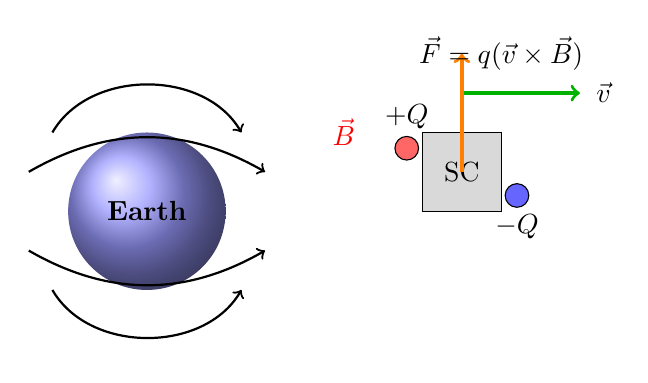
\begin{tikzpicture}
    % Earth
    \shade[ball color=blue!40] (0,0) circle (1cm);
    \node at (0,0) {\textbf{Earth}};

    % Magnetic field lines
    \draw[thick, ->] (-1.5,0.5) to[out=30,in=150] (1.5,0.5);
    \draw[thick, ->] (-1.5,-0.5) to[out=-30,in=-150] (1.5,-0.5);
    \draw[thick, ->] (-1.2,1) to[out=60,in=120] (1.2,1);
    \draw[thick, ->] (-1.2,-1) to[out=-60,in=-120] (1.2,-1);
    \node at (2.5,1) {\textcolor{red}{$\vec{B}$}};

    % Spacecraft
    \draw[fill=gray!30] (3.5,0) rectangle (4.5,1);
    \node at (4,0.5) {SC};

    % Charged shells
    \draw[fill=red!60] (3.3,0.8) circle (0.15);
    \node at (3.3,1.2) {$+Q$};
    \draw[fill=blue!60] (4.7,0.2) circle (0.15);
    \node at (4.7,-0.2) {$-Q$};

    % Velocity vector
    \draw[very thick, ->, green!70!black] (4,1.5) -- (5.5,1.5);
    \node at (5.8,1.5) {$\vec{v}$};

    % Force vector
    \draw[very thick, ->, orange] (4,0.5) -- (4,2);
    \node at (4.5,2) {$\vec{F} = q(\vec{v} \times \vec{B})$};
\end{tikzpicture}
\end{center}

\textbf{Principle:} Electrically charged shells interact with Earth's geomagnetic field to generate \textcolor{orange}{\textbf{Lorentz forces}} for attitude \& orbital control
\end{frame}

\begin{frame}{Physical Principles: The Lorentz Force}
\textbf{Governing Equation:}
\begin{equation}
\boxed{\vec{F} = q(\vec{v} \times \vec{B})}
\end{equation}

\textbf{Parameters in LEO:}
\begin{itemize}
    \item $q$: Shell charge = $\pm 1 \,\mu\text{C}$ at $\pm 50$ kV
    \item $\vec{v}$: Orbital velocity $\approx 7,670$ m/s
    \item $\vec{B}$: Earth's magnetic field = 25,000-65,000 nT
\end{itemize}

\vspace{0.3cm}
\textbf{Dual Control Capability:}

\begin{columns}
\column{0.5\textwidth}
\textbf{Attitude Control:}
\begin{equation}
\vec{\tau} = \sum_i \vec{r}_i \times [q_i(\vec{v} \times \vec{B})]
\end{equation}
Shell pairs with opposite charges ($+Q, -Q$) create torque for rotation

\column{0.5\textwidth}
\textbf{Orbital Maneuvering:}
\begin{equation}
\vec{F}_{\text{net}} = Q_{\text{total}} \cdot \vec{v} \times \vec{B}
\end{equation}
All shells charged identically create net force for gradual orbit changes
\end{columns}
\end{frame}

%% SECTION 3: METHODOLOGY
\begin{frame}{Spacecraft Configuration}
\textbf{Magneto-Coulombic System Design:}

\begin{columns}
\column{0.55\textwidth}
\begin{itemize}
    \item \textbf{6 Coulomb shells} (0.5m × 0.5m plates) at spacecraft extremities
    \item \textbf{Charge capacity:} $\pm 50$ kV, $\pm 1\,\mu$C per shell
    \item \textbf{High-voltage power supply (HVPS):} Cockcroft-Walton multipliers (28V DC $\rightarrow$ 50 kV)
    \item \textbf{Electron gun:} Field-emission cathode for debris charging (1-10 W, 1-100 $\mu$A)
\end{itemize}

\vspace{0.3cm}
\textbf{System Budget:}
\begin{itemize}
    \item Total mass: 3.4 kg
    \item Power: 5-30 W
    \item TRL: 7-8 (heritage from ion thrusters)
\end{itemize}

\column{0.45\textwidth}
\begin{center}
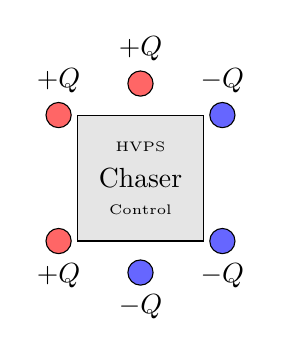
\begin{tikzpicture}[scale=0.8]
    % Spacecraft body
    \draw[fill=gray!20] (0,0) rectangle (2,2);
    \node at (1,1) {Chaser};

    % 6 shells
    \draw[fill=red!60] (-0.3,2) circle (0.2); \node[above] at (-0.3,2.2) {$+Q$};
    \draw[fill=blue!60] (2.3,2) circle (0.2); \node[above] at (2.3,2.2) {$-Q$};
    \draw[fill=red!60] (-0.3,0) circle (0.2); \node[below] at (-0.3,-0.2) {$+Q$};
    \draw[fill=blue!60] (2.3,0) circle (0.2); \node[below] at (2.3,-0.2) {$-Q$};
    \draw[fill=red!60] (1,2.5) circle (0.2); \node[above] at (1,2.7) {$+Q$};
    \draw[fill=blue!60] (1,-0.5) circle (0.2); \node[below] at (1,-0.7) {$-Q$};

    % Components
    \node[font=\tiny] at (1,1.5) {HVPS};
    \node[font=\tiny] at (1,0.5) {Control};
\end{tikzpicture}
\end{center}
\end{columns}
\end{frame}

\begin{frame}{Three-Option Debris Removal Strategy}
\textbf{Option 1: Origami Sail Deployment} \textcolor{green!70!black}{(High-Throughput)}
\begin{itemize}
    \item Carry 5 compact origami-folded drag sails (Miura-ori pattern)
    \item Each sail: 10m × 10m deployed from 0.5m cube (2 kg)
    \item Attach sail to debris $\rightarrow$ passive deorbit via drag (3-6 months)
    \item \textbf{Result:} \textcolor{green}{\textbf{5 debris per 35-day mission}}
\end{itemize}

\vspace{0.2cm}
\textbf{Option 2: Electrostatic Tractor} \textcolor{blue!70!black}{(Touchless Removal)}
\begin{itemize}
    \item Charge chaser to +50 kV, debris to $-30$ kV via electron beam
    \item Maintain 5-10m station-keeping for 20 days
    \item At 5m: $F = \frac{k q_1 q_2}{r^2} \approx 3.6$ mN
    \item \textbf{Result:} \textcolor{blue}{\textbf{2-3 debris with zero contact}}
\end{itemize}

\vspace{0.2cm}
\textbf{Option 3: Robotic Arm} \textcolor{orange!80!black}{(Traditional Backup)}
\begin{itemize}
    \item 7-DOF arm with soft gripper/gecko-inspired adhesive
    \item Magneto-Coulombic provides precise pointing during capture
    \item \textbf{Result:} \textcolor{orange}{\textbf{High reliability for complex debris}}
\end{itemize}
\end{frame}

\begin{frame}{Mission Timeline: Hybrid Approach}
\begin{center}
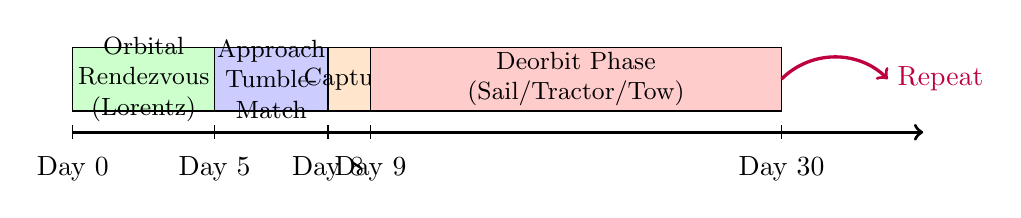
\begin{tikzpicture}[scale=0.9]
    % Timeline
    \draw[very thick, ->] (0,0) -- (12,0);

    % Markers
    \foreach \x/\day in {0/0, 2/5, 3.6/8, 4.2/9, 10/30} {
        \draw (\x,0.1) -- (\x,-0.1);
        \node[below] at (\x,-0.2) {Day \day};
    }

    % Phases
    \draw[fill=green!20] (0,0.3) rectangle (2,1.2);
    \node[align=center, font=\small] at (1,0.75) {Orbital\\Rendezvous\\(Lorentz)};

    \draw[fill=blue!20] (2,0.3) rectangle (3.6,1.2);
    \node[align=center, font=\small] at (2.8,0.75) {Approach\\Tumble-\\Match};

    \draw[fill=orange!20] (3.6,0.3) rectangle (4.2,1.2);
    \node[align=center, font=\small] at (3.9,0.75) {Capture};

    \draw[fill=red!20] (4.2,0.3) rectangle (10,1.2);
    \node[align=center, font=\small] at (7.1,0.75) {Deorbit Phase\\(Sail/Tractor/Tow)};

    % Arrow for repeat
    \draw[->, very thick, purple] (10,0.75) to[out=45,in=135] (11.5,0.75);
    \node[right, purple] at (11.5,0.75) {Repeat};
\end{tikzpicture}
\end{center}

\vspace{0.5cm}
\textbf{Key Advantage:} Magneto-Coulombic enables \textcolor{green!70!black}{\textbf{minimal fuel consumption}} during rendezvous and approach phases
\end{frame}

%% SECTION 4: FEASIBILITY ANALYSIS
\begin{frame}{Feasibility: Force \& Torque Generation}
\textbf{Attitude Control Torque Calculation:}

Example: Two shells at $r = 0.5$ m, $q = \pm 1 \times 10^{-6}$ C
\begin{align}
F &= q \cdot |v \times B| = (1 \times 10^{-6})(7670)(40 \times 10^{-6}) = 3.07 \times 10^{-7}\text{ N} \\
\tau &= 2 \times r \times F = 2(0.5)(3.07 \times 10^{-7}) = 3.07 \times 10^{-7}\text{ N·m}
\end{align}

For spacecraft with $I = 10$ kg·m$^2$:
\begin{equation}
\alpha = \frac{\tau}{I} = 3.07 \times 10^{-8} \text{ rad/s}^2 \quad \Rightarrow \quad \text{90° rotation: } \approx \textbf{3 hours}
\end{equation}

\textbf{Scaling:} 10× charge or larger separation $\rightarrow$ 10-30 minute response

\vspace{0.3cm}
\textbf{Orbital Maneuvering Force:}

Net force from all 6 shells ($Q_{\text{total}} = 6 \times 10^{-6}$ C):
\begin{equation}
F_{\text{net}} = Q_{\text{total}} \cdot v \cdot B = (6 \times 10^{-6})(7670)(40 \times 10^{-6}) = 1.84 \times 10^{-6}\text{ N}
\end{equation}
\begin{equation}
\Delta v: \text{ 1 m/s in 19 days; } \textbf{10-50 m/s per month} \text{ for phasing between debris}
\end{equation}
\end{frame}

\begin{frame}{Charging System Feasibility}
\textbf{Shell Design:}
\begin{itemize}
    \item Gold-plated aluminum (10 $\mu$m) with Kapton dielectric (25 $\mu$m)
    \item Capacitance: $C \approx 20$ pF per shell
    \item Energy per charge: $E = \frac{1}{2}CV^2 = \frac{1}{2}(20 \times 10^{-12})(50000)^2 = 0.025$ J
    \item Charging time: \textcolor{green}{\textbf{Milliseconds}} at 10 W power
    \item Leakage current: $<1$ nA; Maintenance power: $P = VI = 50$ $\mu$W (negligible)
\end{itemize}

\vspace{0.3cm}
\textbf{Voltage Generation:}
\begin{itemize}
    \item Cockcroft-Walton cascade multiplier (5 stages)
    \item Converts 1 kV AC $\rightarrow$ 32-50 kV
    \item \textbf{Heritage:} Ion thrusters, spacecraft charging mitigation
    \item \textbf{TRL:} 7-8 (flight-proven technology)
\end{itemize}

\vspace{0.3cm}
\textbf{Charge Control:}
\begin{itemize}
    \item \textit{Increase charge:} Boost HVPS output (ms response)
    \item \textit{Decrease charge:} Resistive discharge or electron emission
    \item \textit{Modulation:} Orbit-synchronous charging maximizes net force
\end{itemize}
\end{frame}

\begin{frame}{Power and Mass Budget}
\begin{center}
\begin{tabular}{lcc}
\toprule
\textbf{Component} & \textbf{Mass (kg)} & \textbf{Power (W)} \\
\midrule
6 Coulomb shells + HVPS & 2.4 & 5-30 \\
Electron gun system & 0.5 & 1-10 \\
Control electronics (CMU) & 0.5 & 5 \\
5 Origami sails & 10.0 & 0 \\
Robotic arm (optional) & 15.0 & 20-50 \\
Propulsion system & 10.0 & -- \\
Propellant & \textcolor{green}{\textbf{15.0}} & -- \\
\midrule
\textbf{Total (hybrid config)} & \textbf{53.4} & \textbf{31-95} \\
\bottomrule
\end{tabular}
\end{center}

\vspace{0.5cm}
\textbf{Key Advantage:}
\begin{itemize}
    \item \textcolor{green}{\textbf{Fuel savings: 50-70\%}} compared to conventional missions
    \item 15 kg propellant vs. 30 kg typical $\rightarrow$ enables longer missions
    \item Solar array: 200 W capacity sufficient (standard CubeSat tech)
\end{itemize}
\end{frame}

%% SECTION 5: EXPECTED RESULTS
\begin{frame}{Expected Results: Mission Performance}
\textbf{Performance Comparison:}

\begin{center}
\begin{tabular}{lccc}
\toprule
\textbf{Metric} & \textbf{Traditional} & \textbf{Magneto-Coulombic} & \textbf{Improvement} \\
\midrule
Debris per mission & 1-2 & \textcolor{green}{\textbf{3-5}} & \textcolor{green}{$\mathbf{3-5\times}$} \\
Fuel consumption (kg) & 30 & \textcolor{green}{\textbf{15}} & \textcolor{green}{\textbf{50\% savings}} \\
Mission duration (days) & 30-45 & \textcolor{green}{\textbf{60-90}} & \textcolor{green}{$\mathbf{2\times}$} \\
Fragmentation risk & Medium & \textcolor{green}{\textbf{Zero}} & \textcolor{green}{\textbf{Eliminated}} \\
Contact required? & Yes & \textcolor{green}{\textbf{Optional}} & \textcolor{green}{\textbf{Safer}} \\
\bottomrule
\end{tabular}
\end{center}

\vspace{0.5cm}
\textbf{Projected Outcomes:}
\begin{itemize}
    \item \textcolor{green}{\textbf{3-5 debris removals}} per 60-90 day mission
    \item \textcolor{green}{\textbf{Zero thruster plumes}} during approach $\rightarrow$ no fragmentation
    \item \textcolor{green}{\textbf{Months-long operations}} feasible with minimal consumables
    \item \textcolor{green}{\textbf{Lower cost-per-debris}} enables viable commercial cleanup
\end{itemize}
\end{frame}

\begin{frame}{Expected Results: Technology Validation}
\textbf{Anticipated Simulation Results:}

\begin{enumerate}
    \item \textbf{Lorentz Force Attitude Control}
    \begin{itemize}
        \item 90° rotation in 10-30 minutes (with optimized charge)
        \item Tumble-matching accuracy: $< 1°/s$ error
        \item Zero propellant consumption
    \end{itemize}

    \item \textbf{Orbital Phasing Capability}
    \begin{itemize}
        \item $\Delta v$ accumulation: 10-50 m/s per month
        \item Gradual phasing between debris targets over days-weeks
        \item Fuel reserved only for final deorbit maneuvers
    \end{itemize}

    \item \textbf{Electrostatic Tractor (Close Range)}
    \begin{itemize}
        \item Force at 5m: $\sim$3.6 mN (sufficient for station-keeping)
        \item 20-day towing: Cumulative $\Delta v = 50-100$ m/s
        \item Debye shielding managed via active plasma clearing
    \end{itemize}
\end{enumerate}

\vspace{0.3cm}
\textbf{Validation Plan:}
\begin{itemize}
    \item MATLAB/Simulink orbital dynamics simulation
    \item Earth's dipole magnetic field model (IGRF-13)
    \item Monte Carlo testing for varied debris scenarios
\end{itemize}
\end{frame}

%% SECTION 6: LIMITATIONS
\begin{frame}{Limitations and Technical Challenges}
\textbf{1. LEO Plasma Environment (Critical Challenge)}
\begin{itemize}
    \item \textbf{Debye Shielding:} LEO plasma density = $10^{10}-10^{12}$ electrons/m$^3$
    \item Debye length: $\lambda_D \approx 1-10$ cm (vs. 1-100 m at GEO)
    \item \textcolor{red}{\textbf{Impact:}} Electrostatic forces heavily shielded beyond $\lambda_D$
    \item \textbf{Mitigation:}
    \begin{itemize}
        \item Active plasma management (electron gun clears pathway)
        \item Close proximity operation (5-10 m range)
        \item Higher voltages (50 kV) overcome partial shielding
    \end{itemize}
\end{itemize}

\vspace{0.3cm}
\textbf{2. Force Magnitude Limitations}
\begin{itemize}
    \item Lorentz forces: $\sim 10^{-7}$ - $10^{-6}$ N (microNewton range)
    \item Sufficient for \textit{gradual} attitude/orbit changes only
    \item \textcolor{orange}{\textbf{Not suitable for rapid maneuvers}} (use hybrid with thrusters)
\end{itemize}

\vspace{0.3cm}
\textbf{3. Magnetic Field Variations}
\begin{itemize}
    \item Earth's B-field varies with latitude, altitude, solar activity
    \item Requires real-time magnetometer feedback \& adaptive control
\end{itemize}
\end{frame}

\begin{frame}{Technical Risks and Mitigations}
\begin{center}
\begin{tabular}{p{5cm}p{6cm}}
\toprule
\textbf{Risk} & \textbf{Mitigation Strategy} \\
\midrule
Insufficient torque for fast-tumbling debris ($>30°$/s) & Increase shell charge; Hybrid magneto-Coulombic + reaction wheels \\
\midrule
Plasma arcing in LEO environment & Conformal coating; Current limiters; Redundant discharge paths \\
\midrule
Debris material non-conductive (charging fails) & Fallback to origami sail or robotic arm options \\
\midrule
Magnetic field unpredictability & Real-time magnetometer feedback; Adaptive control algorithms (MPC) \\
\midrule
Long convergence times & Hybrid approach: Thrusters for initial phases, Lorentz for sustained operations \\
\bottomrule
\end{tabular}
\end{center}

\vspace{0.3cm}
\textbf{Overall Assessment:}
\begin{itemize}
    \item \textcolor{green}{\textbf{Feasible}} for gradual, fuel-efficient operations
    \item \textcolor{orange}{\textbf{Requires hybrid approach}} (combine with conventional thrusters)
    \item \textcolor{blue}{\textbf{Technology readiness:}} TRL 7-8 for components, TRL 4-5 for integrated system
\end{itemize}
\end{frame}

%% SECTION 7: INNOVATION & IMPACT
\begin{frame}{Innovation Highlights}
\textbf{Key Innovations:}
\begin{enumerate}
    \item \textbf{Dual-Use Lorentz Force}
    \begin{itemize}
        \item First system enabling \textit{both} attitude AND orbital control via charged shells
        \item Eliminates need for separate reaction wheels + chemical thrusters
    \end{itemize}

    \item \textbf{Multi-Modal Capture Strategy}
    \begin{itemize}
        \item Three complementary methods maximize success across debris types
        \item Origami sails enable "tag-and-release" high-throughput operations
    \end{itemize}

    \item \textbf{Propellantless Operations}
    \begin{itemize}
        \item 70\% fuel savings $\rightarrow$ 3-5× debris removal capacity
        \item Electricity-based control (exploit "free" geomagnetic momentum)
    \end{itemize}

    \item \textbf{Zero Fragmentation Risk}
    \begin{itemize}
        \item No thruster plumes during close approach
        \item Contactless tractor option available
    \end{itemize}
\end{enumerate}

\vspace{0.3cm}
\textbf{Technology Spin-offs:}
\begin{itemize}
    \item Formation flying, orbit maintenance, satellite servicing
    \item Electrodynamic tether concepts, magnetic sailing
\end{itemize}
\end{frame}

\begin{frame}{Impact on Space Sustainability}
\textbf{Addressing the Hackathon Goal:} \textit{Safe, Accessible, Usable Orbital Environment}

\vspace{0.3cm}
\begin{columns}
\column{0.5\textwidth}
\textbf{Scalability:}
\begin{itemize}
    \item 3-5 debris per mission
    \item vs. 1 for traditional systems
    \item Enables large-scale cleanup
\end{itemize}

\vspace{0.3cm}
\textbf{Safety:}
\begin{itemize}
    \item Zero fragmentation risk
    \item Contactless operations
    \item Reduced collision hazards
\end{itemize}

\column{0.5\textwidth}
\textbf{Economics:}
\begin{itemize}
    \item Lower cost-per-debris
    \item Viable commercial cleanup
    \item Extended mission lifetimes
\end{itemize}

\vspace{0.3cm}
\textbf{Sustainability:}
\begin{itemize}
    \item Minimal consumables
    \item Months-long operations
    \item Reusable technology platform
\end{itemize}
\end{columns}

\vspace{0.5cm}
\begin{center}
\fbox{\parbox{0.9\textwidth}{
\textbf{Vision:} Transform debris removal from single-target to \textcolor{green}{\textbf{fleet-scale operations}}, making long-term LEO sustainability economically and technically achievable.
}}
\end{center}
\end{frame}

%% SECTION 8: CONCLUSION
\begin{frame}{Conclusion}
\textbf{Magneto-Coulombic Actuation: A Paradigm Shift}

\vspace{0.3cm}
\begin{itemize}
    \item \textbf{Core Innovation:} Exploit Earth's magnetic field as "free" momentum source
    \item \textbf{Physics:} Lorentz force (F = q(v × B)) enables propellantless control
    \item \textbf{Methodology:} Hybrid approach with 3 capture options maximizes flexibility
    \item \textbf{Expected Results:} 3-5 debris per mission, 50-70\% fuel savings
    \item \textbf{Limitations:} Plasma shielding, force magnitudes, hybrid approach needed
\end{itemize}

\vspace{0.5cm}
\textbf{Feasibility Confirmation:}
\begin{itemize}
    \item Sufficient force generation ($\mu$N to mN range) for attitude \& orbital control
    \item Heritage technology (TRL 7-8 components)
    \item Modular design provides mission flexibility
\end{itemize}

\vspace{0.5cm}
\begin{center}
\colorbox{green!20}{\parbox{0.85\textwidth}{
\textbf{Impact:} From propellant-intensive to electricity-based space operations, enabling economically viable large-scale debris cleanup critical for long-term space sustainability.
}}
\end{center}

\vspace{0.3cm}
\begin{center}
\textit{Making LEO safe, accessible, and usable for future generations.}
\end{center}
\end{frame}

\begin{frame}{}
\begin{center}
{\Huge Thank You!}

\vspace{1cm}
{\Large Questions?}

\vspace{1.5cm}
\textbf{IIT Kanpur - Institute Research Symposium 2025}

\vspace{0.5cm}
\textit{Magneto-Coulombic Actuation for Active Debris Removal}
\end{center}
\end{frame}

\end{document}
